%05/02 - Modesto
\chapter{Estructuras de proteínas}
\section{Obtener y trabajar con estructuras de proteínas}
El pintor surrealista belga René Magritte creó una colección de cuadros surrealistas titulada La trahison des images (1928-1929). El más famoso de estos cuadros muestra una pipa humeante con la siguiente leyenda debajo: «Ceci n'est pas une pipe» (Esto no es una pipa). Efectivamente. En realidad es un cuadro de una pipa.
Esto también es extrapolable a la bioinformática: Una imagen de una proteína, o un archivo informático con las coordenadas de una estructura proteica, no constituye la proteína real. Más bien representa \textbf{una} posible conformación de esa proteína.

Incluso las estructuras determinadas experimentalmente tienen dos limitaciones importantes que deben tenerse en cuenta: (1) representan una estructura fija (excepto las basadas en RMN), mientras que las proteínas in vivo son flexibles y dinámicas, y (2) están sujetas a errores experimentales y a menudo contienen regiones de baja confianza. Además, incluso las estructuras macromoleculares determinadas experimentalmente son, hasta cierto punto, modelos con proporciones variables entre los datos experimentales y las predicciones computacionales utilizadas para hacer coincidir los datos experimentales (como difracción de rayos X, mapas de densidad crio-EM, RMN, SAXS, FRET...) con estructuras o modelos conocidos previamente. Es importante señalar que, aunque las estructuras de proteínas pueden ser muy valiosas, debemos ser conscientes de sus limitaciones y aplicaciones.

\section{Determinación experimental de las estructuras de proteínas}
El análisis estructural de las proteínas es crucial para comprender en detalle los mecanismos moleculares que subyacen a sus funciones. Una representación tridimensional facilita la orientación de diversos dominios, motivos o residuos de interés, lo que resulta esencial para comprender variantes poblacionales o patógenas, el diseño de fármacos y la ingeniería de proteínas. Además, las estructuras proteínicas pueden ayudar a predecir la función y las relaciones evolutivas, ya que la conservación estructural es mayor que la conservación secuencial; el espacio de la estructura proteínica es menor que el espacio secuencial. Sin embargo, la obtención de datos estructurales precisos y detallados puede ser un reto técnico y requerir mucho tiempo. Como ya se ha dicho, el modelado de estructuras proteicas suele ser un valioso complemento o una alternativa. Las estructuras obtenidas experimentalmente suelen obtenerse mediante cristalografía de rayos X, resonancia magnética nuclear (RMN) o criomicroscopía electrónica (crioEM).

\subsection{Cristalografía de rayos X o difracción de rayos X de un solo cristal}
La cristalografía de rayos X, también conocida como difracción de rayos X de monocristal, es una técnica utilizada para determinar la estructura atómica de las moléculas dentro de formas cristalinas. Este proceso consiste en crear un cristal de la molécula de interés, que se coloca en un goniómetro y se expone a un haz concentrado de rayos X (Figura \ref{fig:cristallography}). El patrón de difracción resultante producido por los rayos X que atraviesan el cristal permite determinar las posiciones atómicas, los enlaces químicos, el desorden cristalográfico y otros detalles estructurales. La interpretación de la relación entre el patrón de difracción y la densidad de electrones requiere complejos cálculos matemáticos, en particular mediante transformadas de Fourier, para generar un \textit{modelo} tridimensional de la estructura.

\begin{figure}[h]
\centering
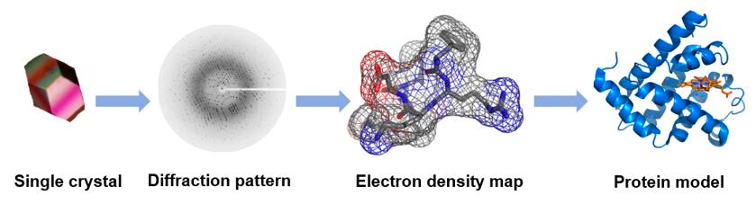
\includegraphics[width = 0.9\textwidth]{figs/paste-F430F5B1.png}
\caption{Flujo de trabajo esquemático de la cristalografía de rayos X. }
\label{fig:cristallography}
\end{figure}

Cuando recogemos datos de difracción de rayos X de un cristal, medimos las intensidades de las ondas difractadas dispersadas en todas las direcciones. Estas medidas nos dan las amplitudes, pero no la información de fase necesaria para reconstruir una imagen (mapa de densidad) de la molécula, lo que se conoce como el \textbf{«problema de fase»}. Este problema se agrava cuando faltan datos o éstos son deficientes. En la cristalografía de proteínas, las fases se obtienen a menudo utilizando las coordenadas atómicas de una proteína similar (reemplazamiento molecular, MR) o identificando las posiciones de los átomos pesados. Los átomos pesados dispersan los rayos X con más intensidad que los ligeros, lo que nos ayuda a determinar sus posiciones dentro del cristal. Comparando los patrones de difracción del cristal original y de uno con átomos pesados añadidos, podemos deducir información de fase mediante la sustitución isomorfa. Los átomos pesados actúan como puntos de referencia para recuperar la información de fase perdida, crucial para reconstruir la estructura tridimensional de la molécula. El reemplazo molecular encuentra modelos que se ajustan a las intensidades experimentales a partir de estructuras conocidas, para lo que suele ser necesario cubrir al menos el 50\% de la estructura total con una d.s.r.m. C$\alpha$ baja. Alrededor del 70\% o más de las estructuras PDB se han resuelto mediante este método (MR), y el número aumenta a medida que se dispone de más estructuras homólogas. Los avances en la predicción de estructuras proteicas de novo han dado lugar a protocolos como MR-Rosetta, QUARK, AWSEM-Suite, I-TASSER-MR y Alphafold-guided MR, que generan estructuras señuelo de tipo nativo útiles para resolver el problema de fase.

La difracción de rayos X es una potente técnica que permite obtener estructuras de alta resolución a nivel atómico de proteínas tanto solubles como de membrana, ya sean apoenzimas o holoenzimas unidas a un sustrato, cofactor o fármaco. Sin embargo, la muestra de proteína debe ser cristalizable (es decir, homogénea), lo que requiere una cantidad sustancial de proteína muy pura. Otra limitación de las estructuras de rayos X es que sólo proporcionan una (o muy pocas) formas estáticas de la proteína, y la localización de los átomos de hidrógeno no puede determinarse mediante métodos de difracción convencionales. Debido a su único electrón, los átomos de hidrógeno son difíciles de detectar con precisión con rayos X, que se dispersan en la densidad de electrones. Aunque los átomos de hidrógeno pueden predecirse, esta limitación sigue complicando algunos análisis químicos. Algunas proteínas conservan toda su funcionalidad, lo que permite realizar experimentos de cristalización con ciertas enzimas, pero también hay numerosos ejemplos en los que la cristalización puede conducir a una representación sesgada de la proteína y dar lugar a artefactos estructurales.

\subsection{Resonancia magnética nuclear}
Todos los núcleos atómicos son partículas cargadas que giran rápidamente y producen frecuencias de resonancia únicas para cada átomo. Cuando se aplica un campo magnético, puede detectarse una señal electromagnética con una frecuencia característica del campo magnético en el núcleo. Este principio constituye la base de la resonancia magnética nuclear (RMN, Figura \ref{fig/rmn}).

\begin{figure}[h]
\centering
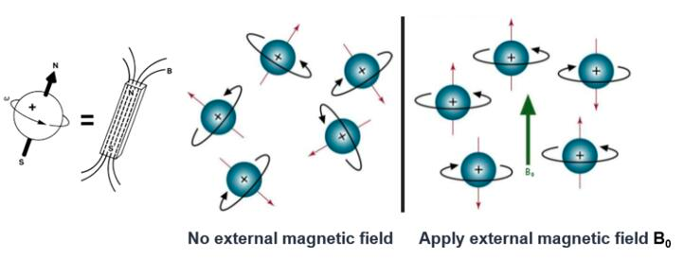
\includegraphics[width = 0.9\textwidth]{figs/paste-2013F0AC.png}
\caption{Bases de la resonancia magnética nuclear.}
\label{fig/rmn}
\end{figure}

Es importante señalar que el movimiento del núcleo no es aislado; interactúa tanto intra como intermolecularmente con los átomos circundantes. Por consiguiente, la espectroscopia de resonancia magnética nuclear puede proporcionar información estructural sobre moléculas específicas. Por ejemplo, en las proteínas, las estructuras secundarias como las $\alpha$-hélices, las $\beta$-hojas y los giros indican diversas disposiciones de los átomos de la cadena principal en el espacio tridimensional. Las distancias entre los núcleos atómicos en estas estructuras secundarias, sus interacciones y las propiedades dinámicas de los segmentos polipeptídicos revelan directamente la estructura tridimensional de las proteínas. Estas características nucleares contribuyen al comportamiento espectroscópico de la muestra, dando lugar a señales de RMN distintivas. La interpretación computacional de estas señales facilita la determinación de la estructura tridimensional de la proteína.

La principal ventaja del método de RMN es que permite medir directamente la estructura tridimensional de las macromoléculas en su estado natural en solución. La RMN proporciona información sobre la dinámica y las interacciones intermoleculares de estas moléculas. La resolución de la estructura tridimensional puede alcanzar el rango subnanométrico. Sin embargo, el espectro de RMN de biomoléculas grandes es complejo y difícil de interpretar, lo que limita su aplicación al análisis de biomoléculas grandes, normalmente por debajo de 20-30 kDa (Figura \ref{fig:molweight}). Además, esta técnica requiere cantidades relativamente grandes de muestras puras (varios miligramos) para lograr una relación señal-ruido razonable.

\begin{figure}[h]
\centering
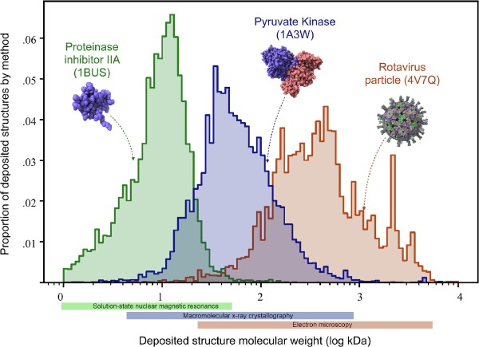
\includegraphics[width = 0.4\textwidth]{figs/paste-FA73AF1E.png}
\caption{Cobertura del peso molecular mediante la técnica estructural. }
\label{fig:molweight}
\end{figure}

\subsection{Criomicroscopía electrónica}
El principio fundamental de la crioEM es la dispersión de electrones, similar a otros métodos de microscopía electrónica. Las muestras se preparan mediante crioconservación antes del análisis. A continuación, se utiliza una fuente de electrones como fuente de luz para medir la muestra. Después de que el haz de electrones atraviese la muestra, un sistema de lentes convierte la señal dispersa en una imagen ampliada que se graba en el detector. Un paso posterior crucial es el procesamiento de la señal, que transforma miles de imágenes de las partículas en diversas orientaciones en una estructura tridimensional de la muestra.

\begin{figure}[h]
\centering
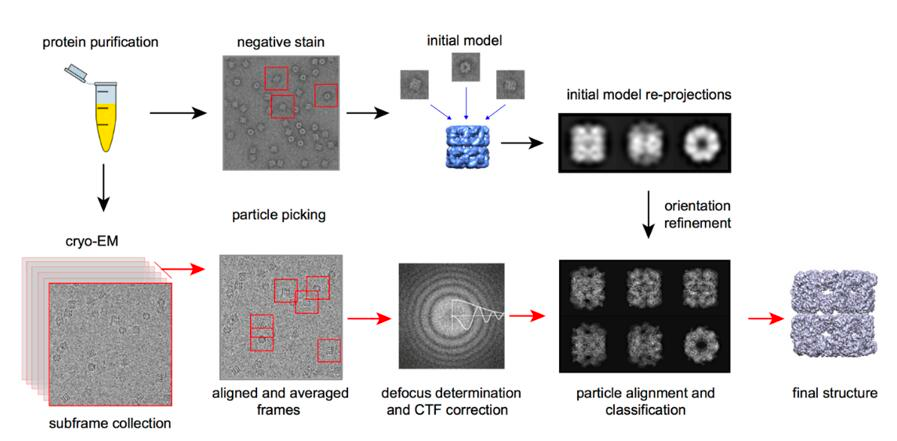
\includegraphics[width = 0.7\textwidth]{figs/paste-5E29F580.png}
\caption{El proceso de la técnica de análisis de partículas individuales Cryo-EM.}
\label{fig:cryoem}
\end{figure}

Tradicionalmente, el uso de métodos de microscopía electrónica para la biología estructural se limitaba a grandes complejos macromoleculares, como las cápsides víricas (Figura \ref{fig:molweight}). Recientemente, también se ha aplicado a partículas más pequeñas. El número de estructuras de proteínas determinadas mediante criomicroscopía electrónica ha aumentado considerablemente en los últimos 5-10 años (consultable en \href{https://www.rcsb.org/stats/all-released-structures}{PDB}). Este aumento se debe a varias mejoras técnicas de la técnica (Figura \ref{fig:cryo-rev}), como la preparación y conservación de muestras, el análisis y el procesamiento, que permiten obtener imágenes a nivel atómico. Estos avances fueron reconocidos con la concesión del Premio Nobel de Química 2017 a Jacques Dubochet, Joachim Frank y Richard Henderson .

\begin{figure}[h]
\centering
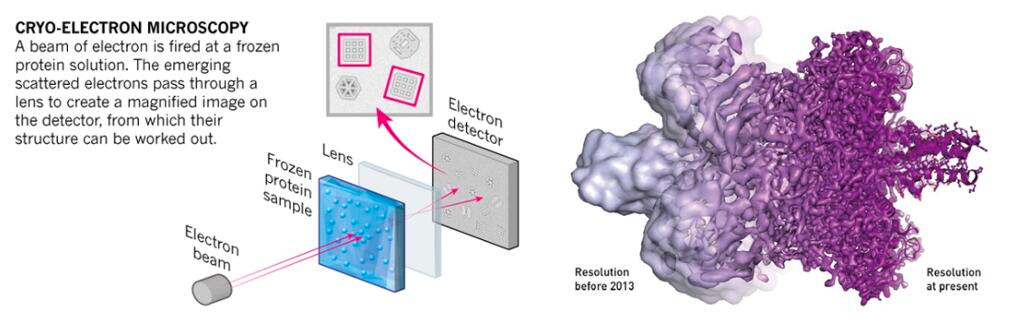
\includegraphics[width = 0.7\textwidth]{figs/paste-E5E5AE75.png}
\caption{La revolución de la criomicroscopía electrónica.}
\label{fig:cryo-rev}
\end{figure}

La crioEM se utiliza habitualmente hoy en día, sobre todo para grandes complejos moleculares o partículas víricas. Permite generar estructuras rápidamente, requiere una cantidad mínima de proteínas y puede producir datos fiables incluso con impurezas presentes. Sin embargo, los microscopios de nueva generación sólo suelen ser asequibles para las grandes instituciones, y las partículas pequeñas suelen tener un alto nivel de ruido. Además, procesar un gran número de imágenes puede suponer un reto cuando se pretende obtener estructuras de alta calidad.

\section{Garantía de calidad estructural}
Toda estructura, independientemente de su origen o método de determinación, es susceptible de error. Las estructuras determinadas experimentalmente son, en realidad, modelos que se han construido para alinearse con los datos experimentales. La calidad de los datos iniciales y la precisión de los procedimientos experimentales influyen significativamente en la fiabilidad de los resultados estructurales. Al igual que ocurre en otras disciplinas científicas, los experimentos independientes pueden dar lugar a modelos relacionados de la misma molécula, aunque suele haber variaciones; no obstante, ambos modelos pueden seguir considerándose representaciones exactas.

\subsection{Parámetros globales en estructuras basadas en experimentos}
Existen distintos parámetros que nos ayudan a comprender la calidad y fiabilidad de una estructura. En primer lugar, la \textbf{resolución} es un buen indicador del nivel de detalle de la estructura, ya que puede afectar en gran medida a la modelización de los datos experimentales.

\begin{figure}[h]
\centering
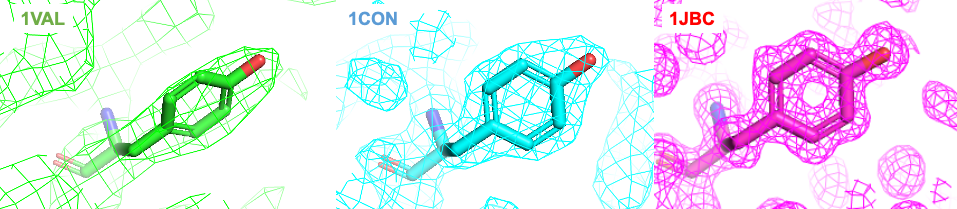
\includegraphics[width = 0.9\textwidth]{figs/paste-C3031EBE.png}
\caption{Efecto de la resolución en la calidad de la densidad electrónica. El residuo Tyr100 de la concanavalina A tal y como se encuentra en las estructuras PDB indicadas a 3 $\AA$, 2 $\AA$ y 1,2 $\AA$. }
\end{figure}

Otro parámetro importante es el \textbf{factor R}, que es la diferencia entre los factores de estructura calculados a partir del modelo y los obtenidos a partir de los datos experimentales. Es decir, el factor R es la desviación entre el patrón de difracción calculado del modelo y el patrón de difracción experimental original. Normalmente, las buenas estructuras con una resolución de 1-3 $\AA$, tienen un factor R de 0,2 (es decir, 20\% de desviación). Sin embargo, debe tenerse en cuenta que este factor suele reducirse tras el refinamiento iterativo, lo que resta importancia a su uso como indicador de fiabilidad. Un factor más fiable es el \textbf{factor$ R_{free}$}. Éste es menos susceptible de manipulación durante el refinamiento, ya que se basa sólo en una pequeña parte de los datos experimentales (5-10\%) que no se utiliza durante la fase de refinamiento.

Una forma más intuitiva, aunque sólo cualitativa, de entender la precisión de las coordenadas de un átomo determinado es el factor B. El valor de temperatura o factor B se correlaciona con los errores de posición, aunque su definición matemática es más compleja. Los valores normales de un factor B se sitúan entre 14 y 30, mientras que los valores superiores a 30 suelen indicar que el átomo se encuentra en una región flexible o desordenada, y los átomos con un factor B superior a 40 suelen descartarse por ser demasiado poco fiables.

La desviación cuadrática media (RMSD) es un estimador tradicional de la calidad de las estructuras resueltas por RMN. Las regiones con valores altos de RMSD (por encima de 6) son las que están menos definidas por los datos. Sin embargo, hay que tener en cuenta que este parámetro también puede ser engañoso, ya que depende en gran medida del procedimiento utilizado para generar y seleccionar los datos que se envían al PDB. Un experimentalista podría reducir la RMSD seleccionando las «mejores» pocas estructuras para su depósito a partir de un borrador mucho mayor. Además, la RMSD tiene muchas otras aplicaciones, como la comparación de diferentes estructuras o modelos de la misma secuencia o de secuencias relacionadas.

En los últimos años, con el aumento de la cantidad y la calidad de las estructuras EM, también se han propuesto nuevos parámetros. Uno de ellos, el \textbf{factor Q}, se introdujo recientemente para la \href{https://www.rcsb.org/news/feature/62de9e5235ec5bb4ddb19a43}{validación de estructuras 3DEM/PDB}. Brevemente, la puntuación del factor Q calcula la resolubilidad de los átomos midiendo la similitud de los valores del mapa alrededor de cada átomo en relación con una función tipo Gauss para un átomo bien resuelto. Una puntuación Q de 1 significa que la similitud es perfecta, mientras que un valor cercano a 0 indica una similitud baja. Si el átomo no está bien situado en el mapa, puede darse un valor Q negativo. Por lo tanto, los valores del factor Q en los informes oscilan entre -1 y +1.

\subsection{Parámetros estereoquímicos}
Dado que todos los modelos estructurales contienen cierto grado de error y que algunos de los parámetros globales de modelización pueden ser controvertidos, podemos analizar la geometría, la estereoquímica y otras propiedades estructurales del modelo para evaluar los modelos estructurales. Estos parámetros comparan una estructura dada con lo que ya se sabe sobre ese tipo de molécula a partir de nuestro conocimiento de las estructuras de alta resolución. Esto significa que las estructuras del espacio estructural actual definen lo que es «normal» en la estructura de una proteína. La ventaja de estos análisis y parámetros derivados es que no tienen en cuenta el proceso que conduce al modelo, sino sólo el producto final y su fiabilidad. La principal desventaja es que el espacio estructural actual se centra en proteínas con función conocida y de interés biomédico o biotecnológico.

Uno de los métodos más comunes y potentes para evaluar la estereoquímica de una proteína es el diagrama de Ramachandran, que se definió en 1963 y sigue utilizándose.

Otro análisis muy utilizado (disponible para todas las estructuras PDB) es el de los \textbf{ángulos de torsión de la cadena lateral}, medidos normalmente como \textbf{valores atípicos de la cadena lateral}. Las cadenas laterales de los aminoácidos también tienen algunas conformaciones preferidas. Al igual que el diagrama de Ramachandran, el diagrama de los ángulos de torsión $\chi$1-$\chi$2 puede indicar problemas con un modelo de proteína si los valores de los ángulos están fuera de los valores de alta densidad.

Los malos contactos o choques indican un modelo deficiente. Es obvio que dos átomos no pueden estar en el mismo lugar (o muy cerca). Podemos definir esto como una situación en la que dos átomos no unidos tienen una distancia entre centros menor que la suma de sus radios de van der Walls.

\section{Visualización de estructuras de proteínas}
\subsection{Formatos de ficheros de estructuras proteicas}
Los datos estructurales experimentales de diferentes métodos se almacenan en diferentes formatos de archivo. Por ejemplo, los datos cristalográficos en bruto suelen almacenarse como archivos \texttt{*.ccp4}, pero los mapas de densidad de Cryo-EM o rayos X pueden almacenarse en archivos \texttt{*.mrc} o \texttt{*.mtz}. Otros formatos de archivo complejos, como el Extensible Markup Language \texttt{*.xml}, proporcionan un marco para estructurar información compleja y documentos como estructuras de proteínas.

Junto con la creación del Banco de Datos de Proteínas, se desarrolló un formato sencillo y estandarizado. El formato Brookhaven o PDB consiste en registros de líneas en un formato fijo que describen coordenadas atómicas, características químicas y bioquímicas, detalles experimentales de la determinación de la estructura y algunas características estructurales como asignaciones de estructuras secundarias, enlaces de hidrógeno o sitios activos. La versión actual se denomina PDBx/mmCIF) también incorpora el formato de archivo de información cristalográfica ampliado (mmCIF), que permite la representación de estructuras de gran tamaño, química compleja y métodos experimentales nuevos e híbridos. Así, los archivos \texttt{*.pdb} y \texttt{*.cif} pueden considerarse idénticos.

\begin{figure}[h]
\centering
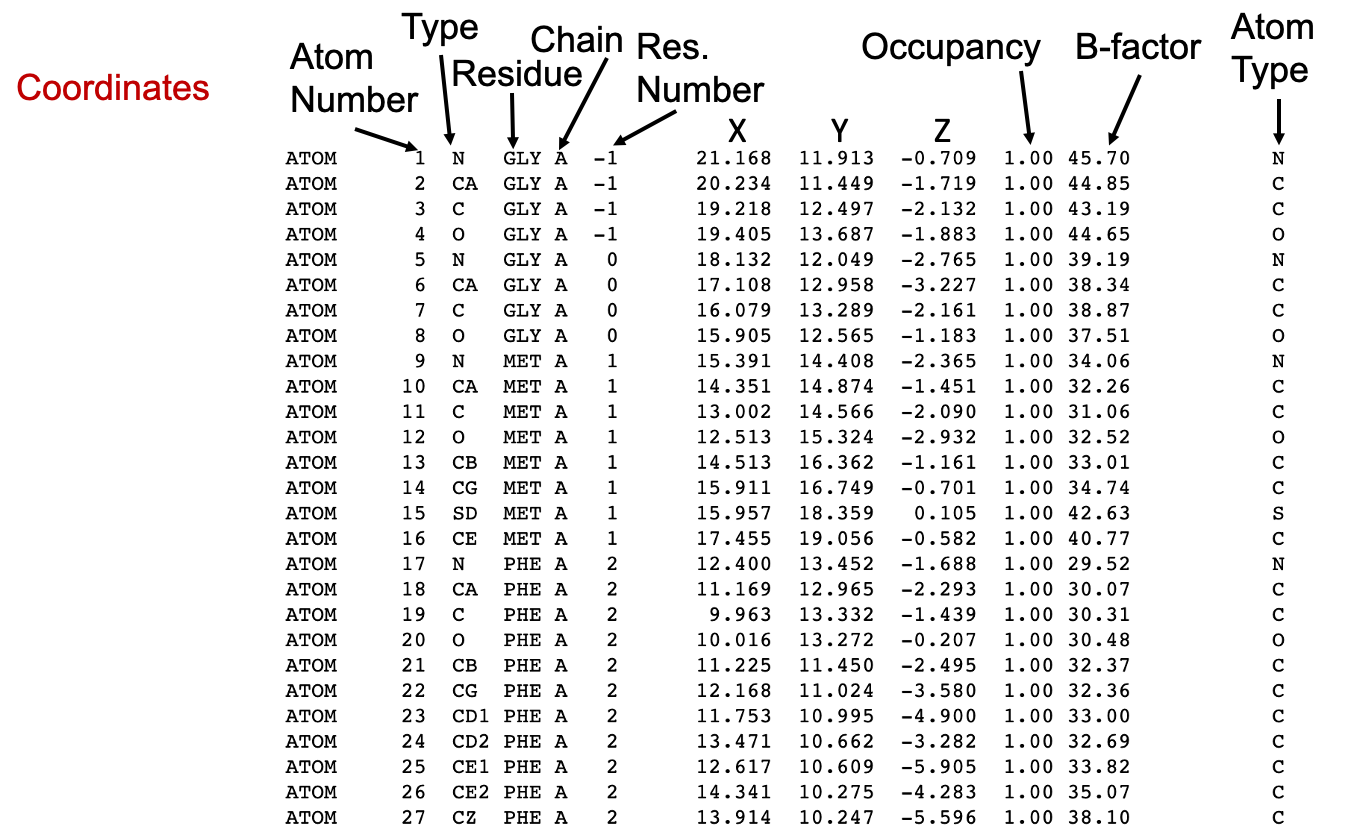
\includegraphics[width = 0.7\textwidth]{figs/coordinates-pdb.png}
\caption{Coordenadas en un fichero PDB.}
\end{figure}

\subsection{Ocupancia y factor B}
Excepto por la repetición del tipo de átomo en la columna de la derecha, las últimas columnas del archivo PDB son la \textbf{ocupancia} y el \textbf{factor de temperatura o el factor B}.

Los cristales macromoleculares están formados por muchas moléculas individuales empaquetadas en una disposición simétrica. En algunos cristales hay ligeras diferencias entre las moléculas individuales. Por ejemplo, una cadena lateral en la superficie puede oscilar entre varias conformaciones, o un sustrato puede unirse en dos orientaciones en un sitio activo, o un ion metálico puede detectarse unido sólo a algunas de las moléculas. Cuando los investigadores construyen el modelo atómico de estas porciones, pueden utilizar la ocupación para estimar la cantidad de cada conformación observada en el cristal. Por tanto, por definición, la suma de los \textbf{valores de ocupación} de cada átomo debe ser 1. Normalmente, vemos un único registro para un átomo, con un valor de ocupación de 1, lo que indica que el átomo se encuentra en todas las moléculas en el mismo lugar del cristal. Sin embargo, si un ion metálico se une sólo a la mitad de las moléculas del cristal, el investigador ve una imagen débil del ion en el mapa de densidad electrónica y puede asignar una ocupación de 0,5 para este átomo en el archivo de estructura PDB. Para cada átomo, se incluyen dos (o más) registros de átomos con ocupaciones tales como 0,5 y 0,5, o 0,4 y 0,6, u otras fracciones de ocupaciones que suman un total de 1.

Por otro lado, el \textbf{valor de temperatura o factor B} es una medida de nuestra confianza en la localización de átomos individuales, como se ha descrito anteriormente. Si encuentra un átomo con un factor de temperatura alto en la superficie de una proteína, tenga en cuenta que es probable que este átomo se mueva mucho y que las coordenadas dadas en el archivo PDB son sólo una posible instantánea de su ubicación. Así, un conjunto de datos de átomos con una ocupación < 1 puede tener un factor B bajo si esa posición es segura. 
Esta columna también es utilizada por los modelos derivados computacionalmente para indicar un valor de confianza que puede ser analizado para diversos fines, incluyendo la coloración de la estructura.

La metionina iniciadora siempre recibe el número de residuo de 1. Sin embargo, como a veces los cortes pueden no ser limpios, puede haber alguna cadena residual anterior a la metionina; estos reciben la numeración 0 y -1.

\subsection{Aplicaciones de visualización de macromoléculas biológicas}
\subsubsection{PyMOL}
PyMOL es un sistema de visualización molecular muy potente escrito originalmente por Warren DeLano. Fue lanzado en 2000 y pronto se hizo muy popular. Actualmente se comercializa bajo licencia de Schrödinger pero se puede solicitar una licencia libre para la enseñanza. Además, el código fuente abierto está disponible en GitHub que se puede instalar en Linux o MAC. 

PyMOL permite trabajar con diferentes representaciones de estructuras, pero también con datos experimentales brutos en diferentes formatos.

PyMOL está escrito en Python y puede ser usado con menús interactivos y también con línea de comandos. Hay muchos recursos que ayudan con PyMOL, como un Wiki de referencia de documentación o un PyMOLWiki soportado por la comunidad. Además, permite la implementación de nuevas funcionalidades como plugins, como PyMod o DockingPie, entre otros. PyMod está diseñado para actuar como interfaz simple e intuitiva entre PyMOL y varias herramientas bioinformáticas (i.e., PSI-BLAST, Clustal Omega, HMMER, MUSCLE, CAMPO, PSIPRED, y MODELLER). Partiendo de la secuencia de aminoácidos de la proteína diana, PyMod está diseñado para llevar a cabo los principales pasos del proceso de modelado homológico (es decir, la búsqueda de plantillas, la alineación de la secuencia diana-plantilla y la construcción del modelo) con el fin de construir un modelo atómico 3D de una proteína diana (o complejo proteico). La integración con PyMOL facilita un análisis detallado del proceso de modelado.

\subsubsection{UCSF ChimeraX}
ChimeraX es un software totalmente de código abierto, desarrollado por la UCSF como versión renovada del antiguo software Chimera, con versiones para Linux, MacOS y Windows. Pretende ser una herramienta integral de biología estructural, pero es más conocido por sus capacidades para mapas EM. Como cualquier otro software de código abierto, en los últimos años ha adquirido nuevas e interesantes capacidades, como la Realidad Virtual o el modelado Alphafold2.

\subsubsection{Estructuras moleculares en su sitio web: Mol* y otros}
LiteMol Viewer es una potente aplicación web HTML5 para la visualización 3D de moléculas y otros datos relacionados. Se utiliza en un navegador web, lo que elimina la necesidad de software externo y también permite la integración con sitios de terceros como un plugin incrustado. 

La misma filosofía se aplica a otros visores de código abierto que se desarrollaron más tarde y que ahora se utilizan más ampliamente, como NGL Viewer y Mol*, utilizados en los sitios RCSB-PDB y PDBe para la visualización 3D de estructuras. Con Mol* puede guardar la sesión de trabajo en formatos \texttt{molj} (sin las estructuras reales) o \texttt{molx} (con estructuras incrustadas).

Por último, para los científicos computacionales, también hay muchas bibliotecas que permiten la representación de moléculas en 3D, como la biblioteca 3Dmol Javascript y su envoltorio Python Py3Dmol, que se puede utilizar en Colab, Jupyter, Quarto o cualquier otro cuaderno Python.

Otra aplicación que se utilizaba, pero que ahora están descatalogada es SwissPDBViewer (también conocida como DeepView), desarrollada para trabajar con la aplicación de modelado homológico SWISS-MODEL. Es una aplicación que proporciona una interfaz fácil de usar que permite analizar varias proteínas al mismo tiempo. Actualmente ha caído en desuso ya que la última versión (4.1) es sólo una aplicación de 32 bits.

